
\section{Discussion}
\label{sec:discuss}

\subsection{Quality}

Our system's rendering quality is directly tied to how many color and
stencil samples the framebuffer maintains per pixel.  This determines the
quality of our antialiasing.  Our GeForce GPUs support up to 16 samples
per pixel while our Quadro GPUs support 32 and 64 samples per pixel as
well.

At 16 samples per pixel, our rendering quality compares quite favorably
with CPU-based path renderers.  Because our GPUs have 8 bits of sub-pixel
precision, irregular coverage sample positions, and our point containment
determinations are numerically sound, we are well-justified in stating
our quality exceeds what can reasonably be expected for CPU-based path
renderers.
We focus on two aspects of path rendering quality where our implementation
has superior quality.

\subsubsection{Stroking Quality}

\begin{figure}[tb]
  %\center{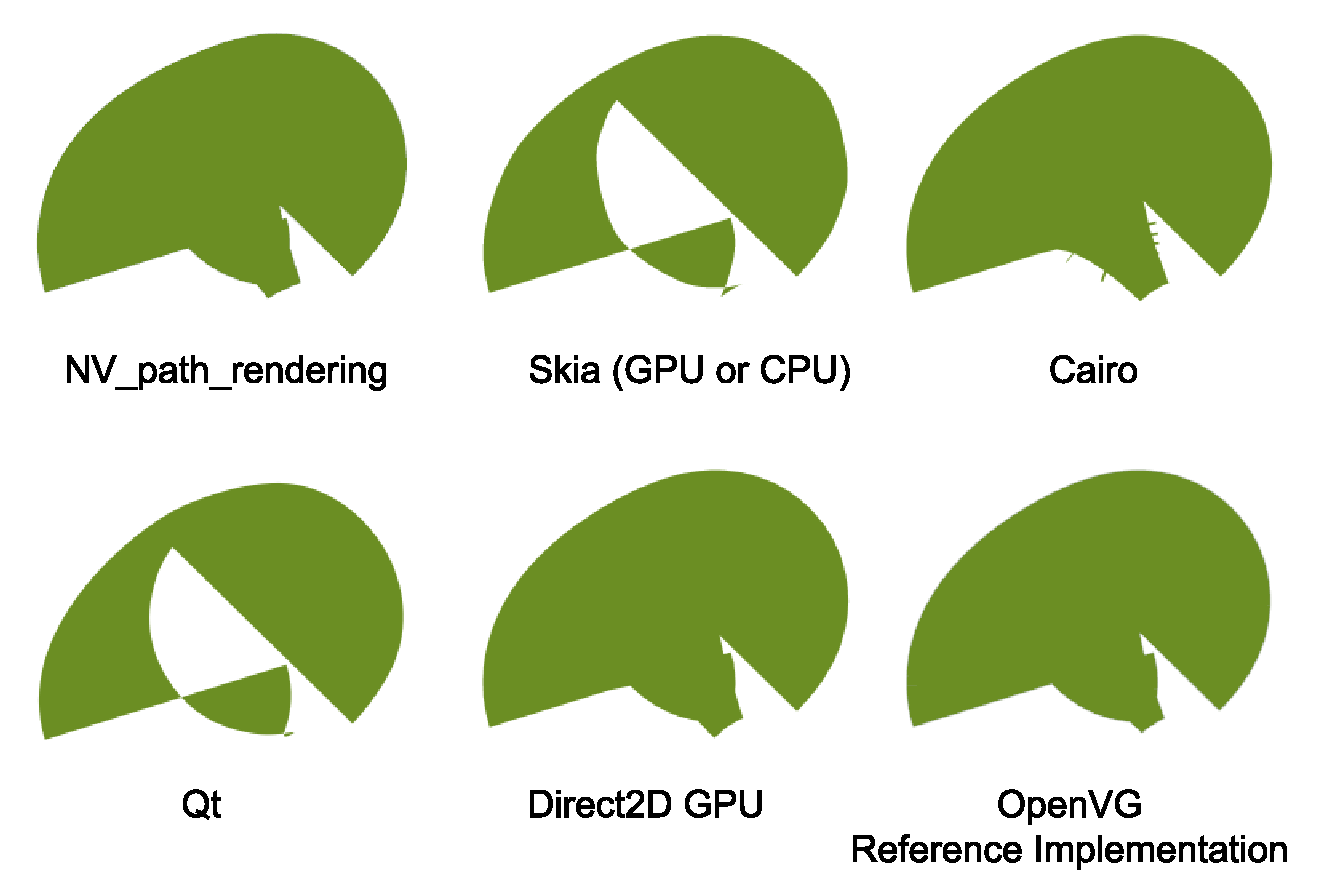
\includegraphics[width=\columnwidth]{stroke_quality.eps}}
  \center{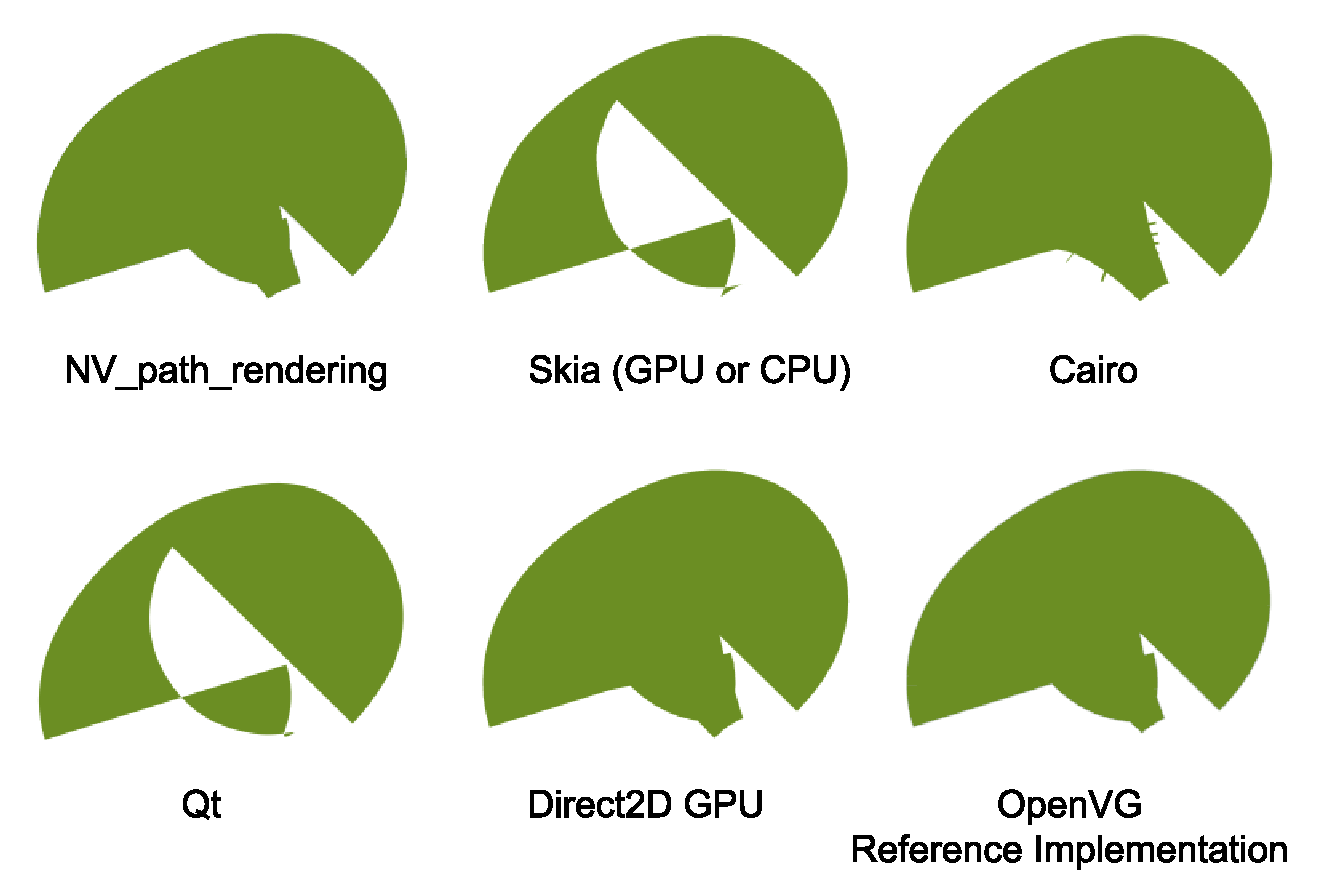
\includegraphics[width=3.1in]{stroke_quality.eps}}
  \caption{\label{fig:stroke-quality} Various path rendering
  implementations drawing a difficult cubic B\'{e}zier curve (the
  centurion head).}
\end{figure}

For stroking, our quadratic B\'{e}zier stroke discard shader is
mathematically consistent with the sweep of an orthogonal pen traversing
the path's trajectory.  In Figure \ref{fig:stroke-quality} we compare
our very fast stroking result to alternatives that are generally
substantially slower on a difficult cubic B\'{e}zier stroke test case.
Notice three path rendering implementation get this test case quite
wrong---whereas {\tt NV\_path\_rendering} matches the OpenVG reference
implementation and Direct2D version.
 
\subsubsection{Conflation Avoidance}

Conflation is an artifact in path rendering systems that occurs when
coverage (a Boolean concept) is {\em conflated} with opacity.  This generally
occurs when sub-pixel coverage is converted to a fractional value and
multiplied into the alpha color component for compositing.  While this
approach is standard practice, it can result in noticeably incorrect
colors.

Conflation is particularly noticeable when two opaque paths {\em exactly} seam
at a shared boundary.  Say path A covers 40\% of the pixel and an adjacent
path B covers the other 60\%.  But if A is drawn first, the pixel picks
up 40\% of A's color and 60\% of the background color.  Now when B is
drawn, the pixel gets 60\% of B's color and 40\% of the combination of
40\% of A's color and 60\% of the background color.  The result is some
fraction of the background color has leaked into the pixel when a more
accurate assessment of coverage would have no background color.

Flash content is particularly prone to conflation artifacts because path
edges are typically authored for exact sharing of edges.  Adobe's Flash
player specifically works to avoid conflation artifacts.  This is possible
because Flash player has complete knowledge of all the paths in a Flash
shape and how those path edges are shared.  Exact sharing of edges is
helpful from a content creation standpoint because a shared edge can be
stored once and used by two paths (more compact) and reduces the overall
layered depth complexity of the scene by avoiding overlaps.
Because {\tt NV\_path\_rendering} maintains distinct sub-pixel color
samples, the scene in Figure \ref{fig:conflation-artifacts} renders free
of conflation artifacts.

\begin{figure}[tb]
  %\center{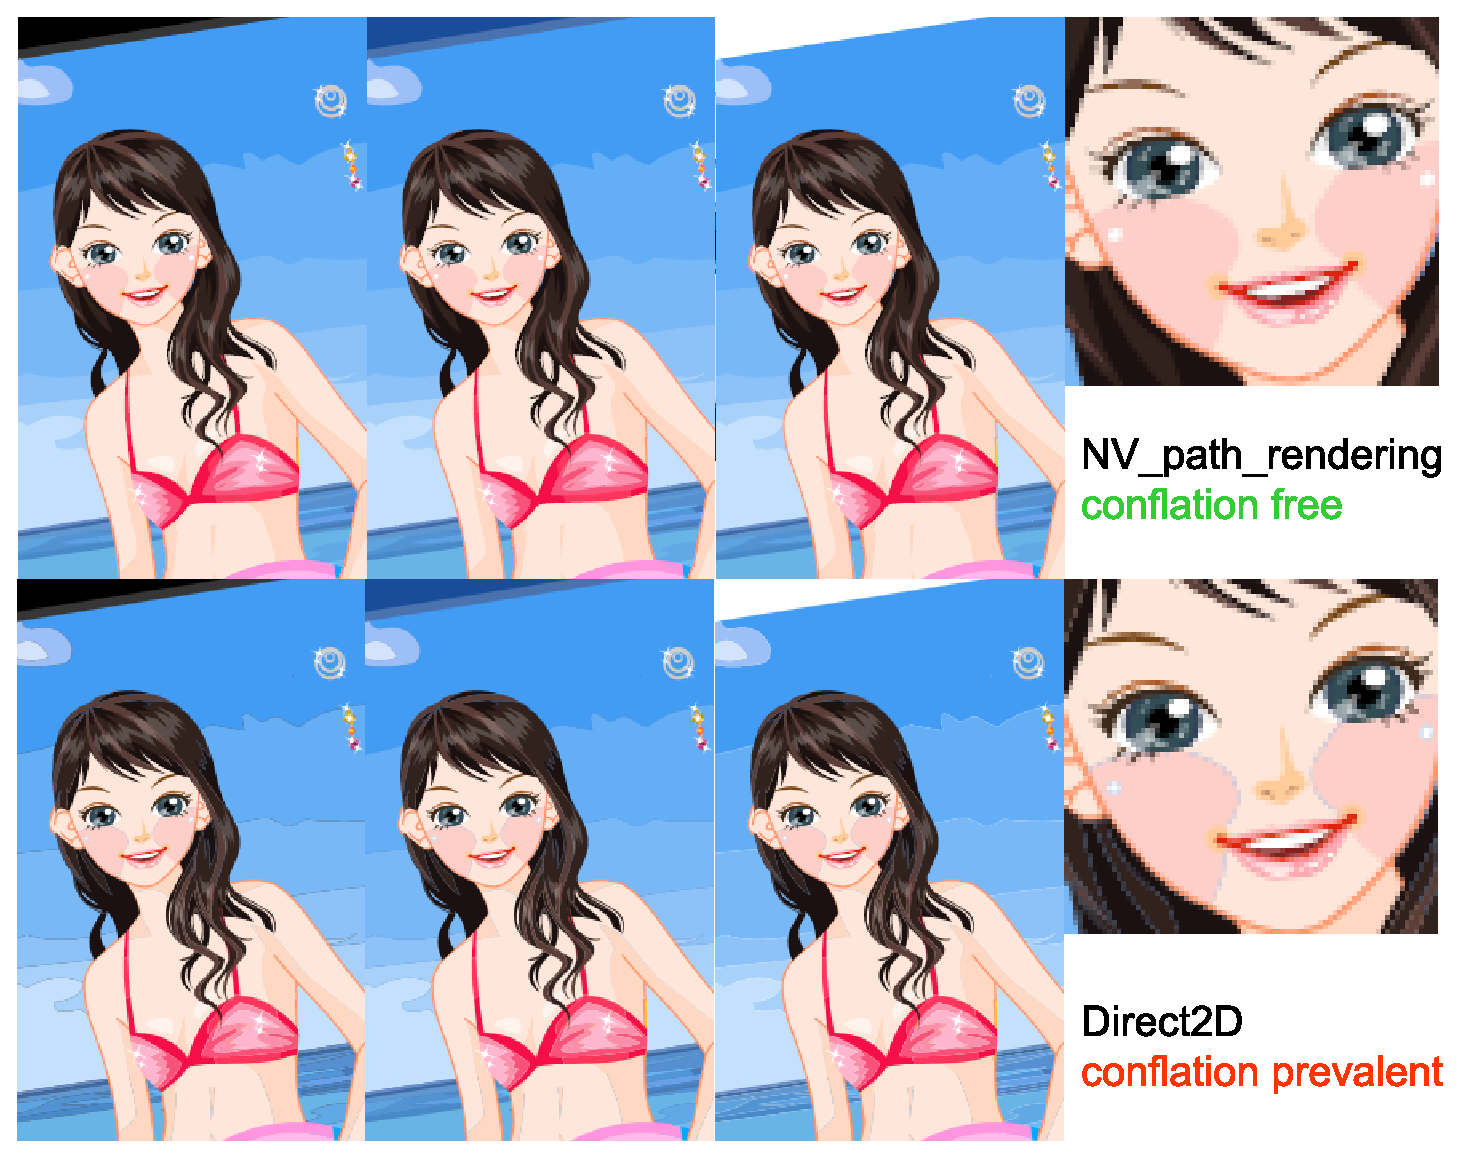
\includegraphics[width=\columnwidth]{conflation_artifacts.eps}}
  \center{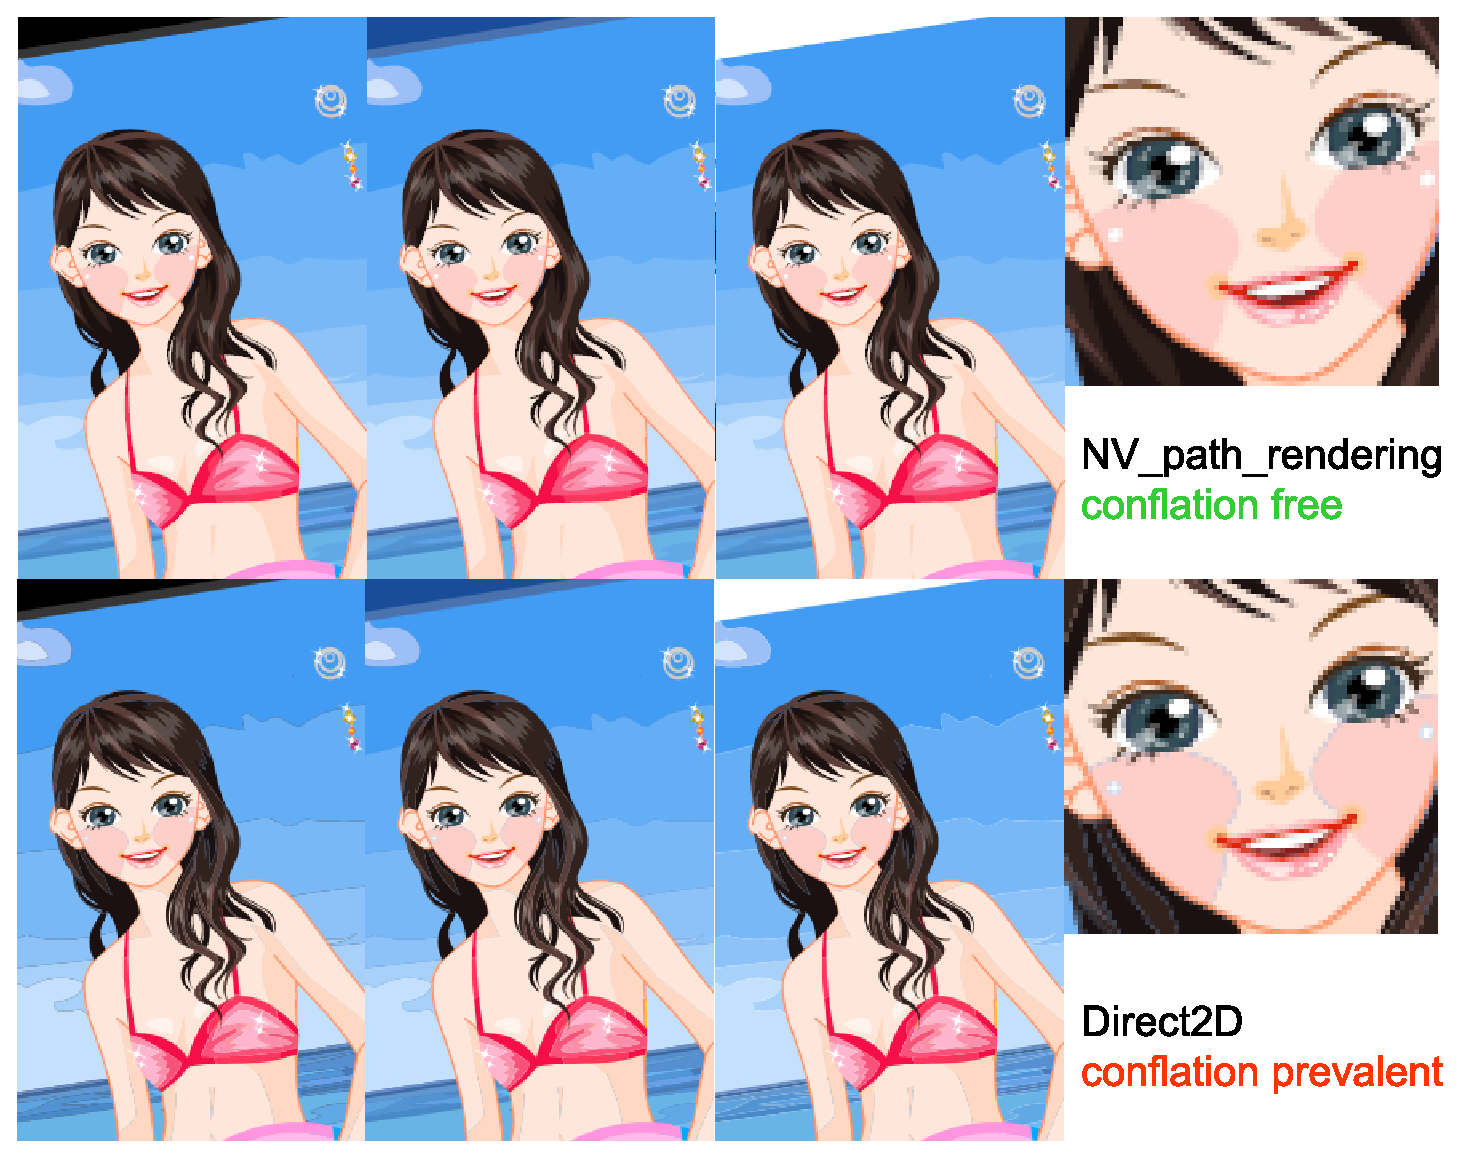
\includegraphics[width=3.3in]{conflation_artifacts.eps}}
  \caption{\label{fig:conflation-artifacts} Flash scene with shared edges.
  {\tt NV\_path\_rendering} shows no conflation while Direct2D (and Cairo,
  Skia, Qt, and OpenVG) shows conflation.  Upper left corner shows the
  background clear color; conflation is tinted by this color in the
  bottom scenes.  Notice the conflated blue tint on the girl's cheek.}
\end{figure}
 
\subsection{Performance}
\label{sec-performance}

The rendering performance of {\tt NV\_path\_rendering} scales with
GPU performance.  Because the baked paths reside on the GPU and are
resolution-independent, once baked, path rendering performance is
decoupled from CPU performance.
Figure \ref{fig:nvpr-performance}
charts the performance of {\tt NV\_path\_rendering} relative to
alternatives---including GPU-accelerated alternatives such as Direct2D and Skia's Ganesh approach.

Our performance advantage is attributable to the overall rendering
and shading performance of our underlying GPUs.  Several aspects are
particularly noteworthy.  Our underlying GPUs support a fast stencil
culling mode so hundreds of pixels can be culled in a single clock if a
coarse grain test can determine the stencil test for all the pixels would
fail.  This mitigates much of what might otherwise seem very inefficient
about the ``stencil, then cover'' approach.  Also stencil processing
generally is very well optimized.  The 8-bit memory transactions during
the stencil and cover steps can often run at memory bus saturating rates.
Our OpenGL driver implementation makes use of a configurable front-end
processor within the GPU---not otherwise accessible to applications---to
transition quickly between the stencil step and cover step and back.  This
avoids the driver performing expensive revalidations of CPU-managed
state so our rendering stays GPU-limited rather than CPU-bottlenecked,
even when presented with otherwise overwhelming numbers of small paths.

\subsection{New Functionality}
\label{sec:newfunc}

Because {\tt NV\_path\_rendering} is integrated into the OpenGL pipeline
and the coverage information is accessible through the stencil buffer,
we are able to implement unconventional algorithms such as mixing path
rendering with arbitrary 3D graphics.

\begin{figure}[bt]
  %\center{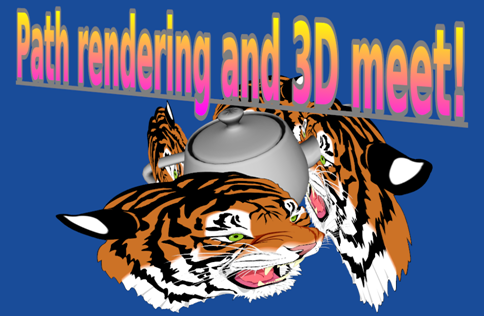
\includegraphics[width=\columnwidth]{tiger3d.png}}
  \center{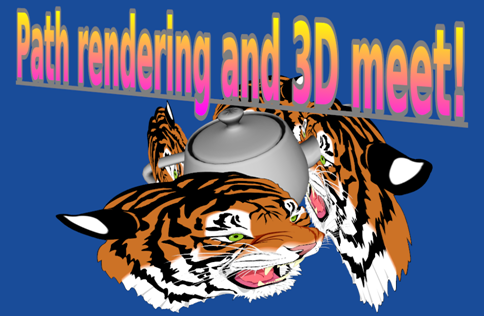
\includegraphics[width=3.3in]{tiger3d.png}}
  \caption{\label{fig:tiger3d} Mixing 3D and path rendering in a single
  window.}
\end{figure}

Figure \ref{fig:tiger3d} demonstrates an example of this capability.
No textures are used in this scene.  Arbitrary zooming into the tigers'
detail is supported.  Notice how the tigers properly occlude each other
and the teapot.  Due to the perspective 3D view, the path rendering is
properly rendered in perspective as well.

